\documentclass[10pt]{article}
\usepackage[utf8]{inputenc}
\usepackage[T1]{fontenc}
\usepackage{amsmath}
\usepackage{amsfonts}
\usepackage{amssymb}
\usepackage[version=4]{mhchem}
\usepackage{stmaryrd}
\usepackage{graphicx}
\usepackage[export]{adjustbox}
\graphicspath{ {./images/} }
\usepackage{bbold}

\begin{document}
\section*{Math 141 Tutorial 5 Solutions}
\section*{Main problems}
\begin{enumerate}
  \item Compute the following integrals using integration by parts (IBP)\\
(a) $\int_{0}^{\ln (2)} s e^{s} \mathrm{~d} s$\\
(e) $\int x \sec ^{2} x \mathrm{~d} x$\\
(b) $\int x \cosh (x) \mathrm{d} x$\\
(f) $\int \arcsin (x) \mathrm{d} x$\\
(c) $\int_{0}^{1} \arctan (x) \mathrm{d} x$\\
(g) $\int \frac{\ln x}{x^{2}} \mathrm{~d} x$\\
(d) $\int_{1}^{e} \ln \left(x^{8}\right) \mathrm{d} x$
\end{enumerate}

Solution:\\
(a) Here we take $u=s$ and $\mathrm{d} v=e^{s} \mathrm{~d} s$. Then, $\mathrm{d} u=\mathrm{d} s$ and $v=e^{s}$. Thus,

$$
\begin{aligned}
\int_{0}^{\ln (2)} s e^{s} \mathrm{~d} s & =\left.s e^{s}\right|_{s=0} ^{s=\ln 2}-\int_{0}^{\ln 2} e^{s} \mathrm{~d} s \\
& =e^{\ln 2} \ln 2-\left(e^{\ln 2}-e^{0}\right) \\
& =2 \ln 2-2+1 \\
& =2 \ln 2-1
\end{aligned}
$$

(b) Take $u=x$ and $\mathrm{d} v=\cosh x \mathrm{~d} x$. Then, $\mathrm{d} u=\mathrm{d} x$ and $v=\sinh x$. Consequently,

$$
\begin{aligned}
\int x \cosh x \mathrm{~d} x & =x \sinh x-\int \sinh x \mathrm{~d} x \\
& =x \sinh x-\cosh x+C \\
& =x \sinh x-\cosh x+C
\end{aligned}
$$

(c) As a first step, We choose $u=\arctan x$ and $\mathrm{d} v=\mathrm{d} x$. This gives

$$
\mathrm{d} u=\frac{1}{1+x^{2}} \mathrm{~d} x \quad \text { and } \quad v=x
$$

Thus, our given integral becomes

$$
\begin{aligned}
\int_{0}^{1} \arctan (x) \mathrm{d} x & =\left.x \arctan (x)\right|_{x=0} ^{x=1}-\int_{0}^{1} \frac{x}{1+x^{2}} \mathrm{~d} x \\
& =\arctan (1)-\int_{0}^{1} \frac{x}{1+x^{2}} \mathrm{~d} x \\
& =\frac{\pi}{4}-\int_{0}^{1} \frac{x}{1+x^{2}} \mathrm{~d} x
\end{aligned}
$$

To handle this second integral that has appeared, we will make the substitution $t=x^{2}+1$.\\
Then, $t(0)=1$ and $t(1)=2$. Furthermore, $\mathrm{d} t=2 x \mathrm{~d} x$ so that

$$
\begin{aligned}
\int_{0}^{1} \frac{x}{1+x^{2}} \mathrm{~d} x & =\int_{1}^{2} \frac{\mathrm{~d} u / 2}{u} \\
& =\frac{1}{2} \int_{1}^{2} \frac{\mathrm{~d} u}{u} \\
& =\frac{1}{2}\left(\left.\ln u\right|_{u=1} ^{u=2}\right) \\
& =\frac{\ln 2}{2}
\end{aligned}
$$

So, to summarize:

$$
\begin{aligned}
\int_{0}^{1} \arctan (x) \mathrm{d} x & =\frac{\pi}{4}-\int_{0}^{1} \frac{x}{1+x^{2}} \mathrm{~d} x \\
& =\frac{\pi}{4}-\frac{\ln 2}{2}
\end{aligned}
$$

(d) Notice that $\ln x^{8}=8 \ln x$. Thus,

$$
\begin{aligned}
\int_{1}^{e} \ln \left(x^{8}\right) \mathrm{d} x & =8 \int_{1}^{e} \ln x \mathrm{~d} x \\
& =8\left[\left.x \ln x\right|_{x=1} ^{x=e}-\int_{1}^{e} \frac{x}{x} \mathrm{~d} x\right] \\
& =8\left[e \ln e-1 \ln 1-\int_{1}^{e} \mathrm{~d} x\right] \\
& =8[e \ln e-e+1] \\
& =8
\end{aligned}
$$

(e) We proceed using IBP. Take $u:=x$ and $\mathrm{d} v=\sec ^{2} x \mathrm{~d} x$. Then, $\mathrm{d} u=\mathrm{d} x$ and $v=\tan x$. Thus,

$$
\begin{aligned}
\int x \sec ^{2} x \mathrm{~d} x & =x \tan x-\int \tan x \mathrm{~d} x \\
& =x \tan x-\ln |\sec x|+C
\end{aligned}
$$

Page 2\\
(f) We proceed via IBP. First, choose $u:=\arcsin x$ and $\mathrm{d} v=\mathrm{d} x$. This gives

$$
\mathrm{d} u=\frac{\mathrm{d} x}{\sqrt{1-x^{2}}} \quad \text { and } \quad v=x
$$

Consequently,

$$
\int \arcsin (x) \mathrm{d} x=x \arcsin x-\int \frac{x \mathrm{~d} x}{\sqrt{1-x^{2}}}
$$

Now, the integral $-\int \frac{x \mathrm{~d} x}{\sqrt{1-x^{2}}}$ is handled with the substitution $t=1-x^{2}$ (which has $\mathrm{d} t=-2 x \mathrm{~d} x):$

$$
\begin{aligned}
\int \frac{x \mathrm{~d} x}{\sqrt{1-x^{2}}} & =-\frac{1}{2} \int \frac{\mathrm{~d} x}{\sqrt{u}} \\
& =-\sqrt{u}+C \\
& =-\sqrt{1-x^{2}}+C
\end{aligned}
$$

To summarize, we have found that

$$
\begin{aligned}
\int \arcsin (x) \mathrm{d} x & =x \arcsin x-\int \frac{x \mathrm{~d} x}{\sqrt{1-x^{2}}} \\
& =x \arcsin x+\sqrt{1-x^{2}}-C \\
& =x \arcsin x+\sqrt{1-x^{2}}+C^{\prime}
\end{aligned}
$$

where $C^{\prime}$ also denotes an arbitrary constant.\\
(g) Here, we instead proceed using IBP. Take $u=\ln x$ and $\mathrm{d} v=\frac{1}{x^{2}} \mathrm{~d} x$. This gives

$$
\mathrm{d} u=\frac{1}{x} \mathrm{~d} x \quad \text { and } \quad v=-\frac{1}{x}
$$

Thus,

$$
\begin{aligned}
\int \frac{\ln x}{x^{2}} \mathrm{~d} x & =-\frac{\ln x}{x}-\int \frac{1}{x}\left(-\frac{1}{x}\right) \mathrm{d} x \\
& =-\frac{\ln x}{x}+\int \frac{1}{x^{2}} \mathrm{~d} x \\
& =-\frac{\ln x}{x}-\frac{1}{x}+C \\
& =-\frac{1+\ln x}{x}+C .
\end{aligned}
$$

\begin{enumerate}
  \setcounter{enumi}{1}
  \item (a) Using integration by parts, prove the following reduction formula:
\end{enumerate}

$$
\int(\ln x)^{n} \mathrm{~d} x=x(\ln x)^{n}-n \int(\ln x)^{n-1} \mathrm{~d} x
$$

(b) Using your result from (a), determine

$$
\int_{1}^{e}(\ln x)^{3} \mathrm{~d} x
$$

Solution:\\
(a) Taking $u=(\ln x)^{n}$ and $\mathrm{d} v=\mathrm{d} x$ gives us that

$$
\mathrm{d} u=\frac{n(\ln x)^{n-1}}{x} \mathrm{~d} x
$$

and we choose $v=x$. Therefore, an integration by parts gives

$$
\begin{aligned}
\int(\ln x)^{n} \mathrm{~d} x & =x(\ln x)^{n}-\int x \cdot \frac{n(\ln x)^{n-1}}{x} \mathrm{~d} x \\
& =x(\ln x)^{n}-n \int(\ln x)^{n-1} \mathrm{~d} x
\end{aligned}
$$

(b) We use the reduction formula from (a) twice:

$$
\begin{aligned}
\int(\ln x)^{3} \mathrm{~d} x & =x(\ln x)^{3}-3 \int(\ln x)^{2} \mathrm{~d} x \\
& =x(\ln x)^{3}-3 x(\ln x)^{2}+6 \int \ln x \mathrm{~d} x \\
& =x(\ln x)^{3}-3 x(\ln x)^{2}+6 x \ln x-6 x+C
\end{aligned}
$$

Then, we use this antiderivative to evaluate

$$
\begin{aligned}
\int_{1}^{e}(\ln x)^{3} \mathrm{~d} x & =x(\ln x)^{3}-3 x(\ln x)^{2}+6 x \ln x-\left.6 x\right|_{1} ^{e} \\
& =(e-3 e+6 e-6 e)-(0-0+0-6) \\
& =-2 e+6 \\
& =2(3-e)
\end{aligned}
$$

\begin{enumerate}
  \setcounter{enumi}{2}
  \item Compute the following trigonometric integrals.\\
(a) $\int_{0}^{\pi / 2} \sin ^{8}(x) \cos ^{5}(x) \mathrm{d} x$\\
(d) $\int \sin ^{2}(x) \cos ^{4}(x) \mathrm{d} x$\\
(b) $\int \sin ^{5}(x) \mathrm{d} x$\\
(e) $\int \tan ^{3}(x) \sec (x) d x$\\
(c) $\int_{-\pi / 4}^{0} \tan ^{3}(x) \sec ^{4}(x) \mathrm{d} x$\\
(f) $\int_{0}^{\pi / 10} \cos ^{4}(5 x) \mathrm{d} x$
\end{enumerate}

Solution:\\
(a) With the substitution $u:=\sin (x)$, we obtain

$$
\begin{aligned}
\int_{0}^{\pi / 2} \sin ^{8}(x) \cos ^{5}(x) \mathrm{d} x & =\int_{0}^{\pi / 2} \sin ^{8}(x)\left(\cos ^{2}(x)\right)^{2} \cos (x) \mathrm{d} x \\
& =\int_{0}^{\pi / 2} \sin ^{8}(x)\left(1-\sin ^{2}(x)\right)^{2} \underbrace{\cos (x) \mathrm{d} x}_{\mathrm{d} u} \\
& =\int_{0}^{1} u^{8}\left(1-u^{2}\right)^{2} \mathrm{~d} u
\end{aligned}
$$

Then, we can evaluate this last integral after distributing:

$$
\int_{0}^{1} u^{8}\left(1-u^{2}\right)^{2} \mathrm{~d} u=\int_{0}^{1}\left(u^{8}-2 u^{10}+u^{12}\right) \mathrm{d} u=\frac{1}{9}-\frac{2}{11}+\frac{1}{13}=\frac{8}{1287}
$$

(b) We wish to use the substitution $u:=\cos (x)$. To this end, we write

$$
\int \sin ^{5}(x) \mathrm{d} x=\int\left(\sin ^{2}(x)\right)^{2} \sin (x) \mathrm{d} x=\int\left(1-\cos ^{2}(x)\right)^{2} \underbrace{\sin (x) \mathrm{d} x}_{-\mathrm{d} u}
$$

Substituting then yields

$$
\begin{aligned}
\int \sin ^{5}(x) \mathrm{d} x=-\int\left(1-u^{2}\right)^{2} \mathrm{~d} u & =-\int\left(1-2 u^{2}+u^{4}\right) \mathrm{d} u \\
& =-\left(u-\frac{2}{3} u^{3}+\frac{1}{5} u^{5}\right)+C \\
& =-\left(\cos (x)-\frac{2}{3} \cos ^{3}(x)+\frac{1}{5} \cos ^{5}(x)\right)+C
\end{aligned}
$$

(c) In order to utilize the substitution $u:=\tan (x)$, we write

$$
\begin{aligned}
\int_{-\pi / 4}^{0} \tan ^{3}(x) \sec ^{4}(x) \mathrm{d} x & =\int_{-\pi / 4}^{0} \tan ^{3}(x) \sec ^{2}(x) \sec ^{2}(x) \mathrm{d} x \\
& =\int_{-\pi / 4}^{0} \tan ^{3}(x)\left(1+\tan ^{2}(x)\right) \underbrace{\sec ^{2}(x) \mathrm{d} x}_{\mathrm{d} u}
\end{aligned}
$$

We can now substitute to obtain

$$
\begin{aligned}
\int_{-\pi / 4}^{0} \tan ^{3}(x) \sec ^{4}(x) \mathrm{d} x=\int_{-1}^{0} u^{3}\left(1+u^{2}\right) \mathrm{d} u & =\int_{-1}^{0}\left(u^{3}+u^{5}\right) \mathrm{d} u \\
& =-\frac{1}{4}-\frac{1}{6}=-\frac{5}{12}
\end{aligned}
$$

(d) We begin by using trigonometric identities to simplify the integrand. We have

$$
\begin{aligned}
\sin ^{2}(x) \cos ^{4}(x) & =(\sin (x) \cos (x))^{2} \cos ^{2}(x) \\
& =\left(\frac{1}{2} \sin (2 x)\right)^{2}\left(\frac{1+\cos (2 x)}{2}\right) \\
& =\frac{1}{8} \sin ^{2}(2 x)(1+\cos (2 x)) \\
& =\frac{1}{8}\left(\frac{1-\cos (4 x)}{2}\right)(1+\cos (2 x)) \\
& =\frac{1}{16}(1+\cos (2 x)-\cos (4 x)-\cos (4 x) \cos (2 x)) \\
& =\frac{1}{16}\left(1+\cos (2 x)-\cos (4 x)-\frac{\cos (2 x)+\cos (6 x)}{2}\right)
\end{aligned}
$$

Hence

$$
\begin{aligned}
\int \sin ^{2}(x) \cos ^{4}(x) \mathrm{d} x & =\frac{1}{16} \int\left(1+\cos (2 x)-\cos (4 x)-\frac{\cos (2 x)+\cos (6 x)}{2}\right) \mathrm{d} x \\
& =\frac{1}{32} \int(2+\cos (2 x)-2 \cos (4 x)-\cos (6 x)) \mathrm{d} x \\
& =\frac{1}{32}\left(2 x+\frac{1}{2} \sin (2 x)-\frac{1}{2} \sin (4 x)-\frac{1}{6} \sin (6 x)\right)+C \\
& =\frac{1}{192}(12 x+3 \sin (2 x)-3 \sin (4 x)-\sin (6 x))
\end{aligned}
$$

(e) With the substitution $u:=\sec (x)$, we obtain

$$
\begin{aligned}
\int \tan ^{3}(x) \sec (x) \mathrm{d} x & =\int \tan ^{2}(x) \tan (x) \sec (x) \mathrm{d} x \\
& =\int\left(\sec ^{2}-1\right) \underbrace{\tan (x) \sec (x) \mathrm{d} x}_{\mathrm{d} u} \\
& =\int\left(u^{2}-1\right) \mathrm{d} u \\
& =\frac{1}{3} u^{3}-u+C \\
& =\frac{1}{3} \sec ^{3}(x)-\sec (x)+C
\end{aligned}
$$

(f) We begin with the simple substitution $u=5 x$ to simplify the integral:

$$
\int_{0}^{\pi / 10} \cos ^{4}(5 x) \mathrm{d} x=\frac{1}{5} \int_{0}^{\pi / 2} \cos ^{4}(u) \mathrm{d} u
$$

Then, we use trigonometric identities to simplify the integrand:

$$
\begin{aligned}
\cos ^{4}(u)=\left(\cos ^{2}(u)\right)^{2} & =\left(\frac{\cos (2 u)+1}{2}\right)^{2} \\
& =\frac{1}{4}\left(\cos ^{2}(2 u)+2 \cos (2 u)+1\right) \\
& =\frac{1}{4}\left(\frac{\cos (4 u)+1}{2}+2 \cos (2 u)+1\right) \\
& =\frac{1}{8}(\cos (4 u)+4 \cos (2 u)+3)
\end{aligned}
$$

We conclude that

$$
\begin{aligned}
\int_{0}^{\pi / 10} \cos ^{4}(5 x) \mathrm{d} x=\frac{1}{5} \int_{0}^{\pi / 2} \cos ^{4}(u) \mathrm{d} u & =\frac{1}{40} \int_{0}^{\pi / 2}(\cos (4 u)+4 \cos (2 u)+3) \mathrm{d} u \\
& =\frac{1}{40}\left[\frac{1}{4} \sin (4 u)+2 \sin (2 u)+3 u\right]_{0}^{\pi / 2} \\
& =\frac{1}{40}\left[3 \cdot \frac{\pi}{2}\right]=\frac{3 \pi}{80}
\end{aligned}
$$

\begin{enumerate}
  \setcounter{enumi}{3}
  \item Compute the integrals below using Trigonometric Substitution\\
(a) $\int \frac{\sqrt{2-x^{2}}}{x^{2}} \mathrm{~d} x$\\
(c) $\int \sqrt{7+6 x-x^{2}} \mathrm{~d} x$\\
(b) $\int_{\sqrt{3}}^{2} \frac{\sqrt{x^{2}-3}}{x} \mathrm{~d} x$\\
(d) $\int_{0}^{a} x^{2} \sqrt{a^{2}-x^{2}} \mathrm{~d} x$
\end{enumerate}

Solution:\\
(a) The trigonometric substitution we will use is:\\
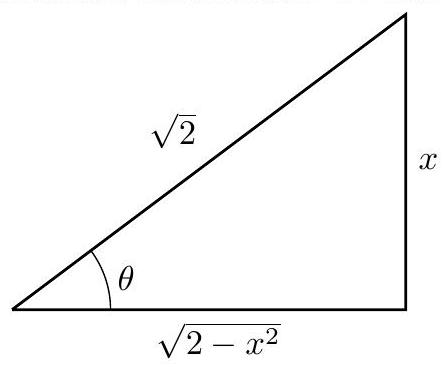
\includegraphics[max width=\textwidth, center]{2024_12_27_c5f2eac2dd536f5b8840g-08(1)}

$$
\begin{aligned}
& \sqrt{2} \sin \theta=x \\
& \sqrt{2} \cos \theta \mathrm{~d} \theta=\mathrm{d} x \\
& \sqrt{2} \cos \theta=\sqrt{2-x^{2}} \\
& \cot \theta=\frac{\sqrt{2-x^{2}}}{x}
\end{aligned}
$$

With this, we have

$$
\begin{aligned}
\int \frac{\sqrt{2-x^{2}}}{x^{2}} \mathrm{~d} x & =\int \frac{\sqrt{2} \cos \theta}{(\sqrt{2} \sin \theta)^{2}} \sqrt{2} \cos \theta \mathrm{~d} \theta \\
& =\int \frac{\cos ^{2} \theta}{\sin ^{2} \theta} \mathrm{~d} \theta \\
& =\int \frac{1-\sin ^{2} \theta}{\sin ^{2} \theta} \mathrm{~d} \theta \\
& =\int\left(\csc ^{2} \theta-1\right) \mathrm{d} \theta \\
& =-\cot \theta-\theta+C \\
& =-\frac{\sqrt{2-x^{2}}}{x}-\arcsin \left(\frac{x}{\sqrt{2}}\right)+C
\end{aligned}
$$

Note: if we instead use the substitution $x=\sqrt{2} \cos \theta$, then we obtain an equivalent solution:

$$
\int \frac{\sqrt{2-x^{2}}}{x^{2}} \mathrm{~d} x=-\frac{\sqrt{2-x^{2}}}{x}+\arccos \left(\frac{x}{\sqrt{2}}\right)+\widetilde{C}
$$

(b) The trigonometric substitution we will use is:\\
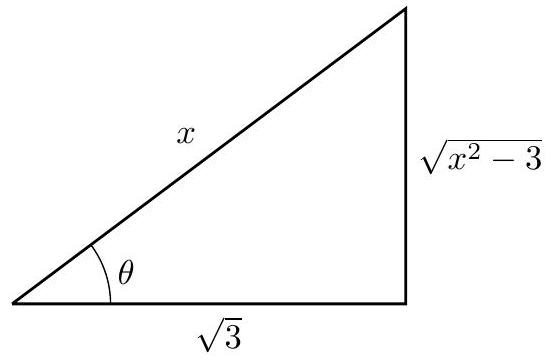
\includegraphics[max width=\textwidth, center]{2024_12_27_c5f2eac2dd536f5b8840g-08}

$$
\begin{aligned}
& \sqrt{3} \sec \theta=x \\
& \sqrt{3} \sec \theta \tan \theta \mathrm{~d} \theta=\mathrm{d} x \\
& \sqrt{3} \tan \theta=\sqrt{x^{2}-3}
\end{aligned}
$$

When $x=\sqrt{3}$ we have $\sec \theta=1$ so $\theta=\operatorname{arcsec}(1)=0$. Similarly, when $x=2$ we have $\sec \theta=\frac{2}{\sqrt{3}}$ so $\theta=\pi / 6$. With this, we have

$$
\begin{aligned}
\int_{\sqrt{3}}^{2} \frac{\sqrt{x^{2}-3}}{x} \mathrm{~d} x & =\int_{0}^{\pi / 6} \frac{\sqrt{3} \tan \theta}{\sqrt{3} \sec \theta} \sqrt{3} \sec \theta \tan \theta \mathrm{~d} \theta \\
& =\sqrt{3} \int_{0}^{\pi / 6} \tan ^{2} \theta \mathrm{~d} \theta \\
& =\sqrt{3} \int_{0}^{\pi / 6}\left(\sec ^{2} \theta-1\right) \mathrm{d} \theta \\
& =\sqrt{3}[\tan \theta-\theta]_{0}^{\pi / 6} \\
& =\sqrt{3}\left(\frac{1}{\sqrt{3}}-\frac{\pi}{6}\right)=1-\frac{\sqrt{3} \pi}{6}
\end{aligned}
$$

(c) As a first step, we observe that

$$
\sqrt{7+6 x-x^{2}}=\sqrt{16-(x-3)^{2}}
$$

We therefore use the following trigonometric substitution:\\
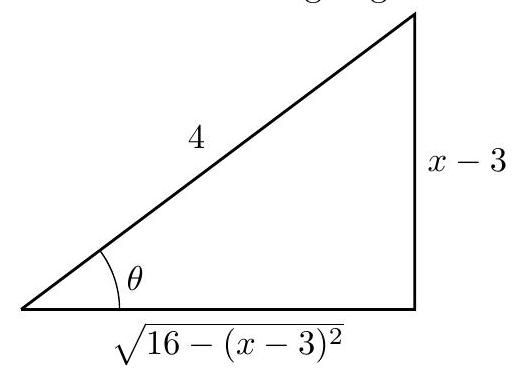
\includegraphics[max width=\textwidth, center]{2024_12_27_c5f2eac2dd536f5b8840g-09}

$$
\begin{aligned}
& 4 \sin \theta=x-3 \\
& 4 \cos \theta \mathrm{~d} \theta=\mathrm{d} x \\
& 4 \cos \theta=\sqrt{16-(x-3)^{2}}
\end{aligned}
$$

We then have

$$
\begin{aligned}
\int \sqrt{7+6 x-x^{2}} \mathrm{~d} x & =\int \sqrt{16-(x-3)^{2}} \mathrm{~d} x \\
& =\int 4^{2} \cos ^{2} \theta \mathrm{~d} \theta \\
& =8 \int(1+\cos (2 \theta)) \mathrm{d} \theta \\
& =8\left(\theta+\frac{1}{2} \sin (2 \theta)\right) \\
& =8\left(\arcsin \left(\frac{x-3}{4}\right)+\sin (\theta) \cos (\theta)\right) \\
& =8\left(\arcsin \left(\frac{x-3}{4}\right)+\frac{(x-3) \sqrt{16-(x-3)^{2}}}{4^{2}}\right) \\
& =8 \arcsin \left(\frac{x-3}{4}\right)+\frac{1}{2}(x-3) \sqrt{7+6 x-x^{2}}
\end{aligned}
$$

Page 9\\
(d) For this last problem, we use the following trigonometric substitution:\\
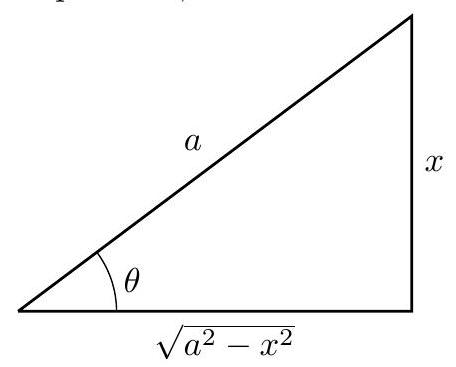
\includegraphics[max width=\textwidth, center]{2024_12_27_c5f2eac2dd536f5b8840g-10}

$$
\begin{aligned}
& a \sin \theta=x \\
& a \cos \theta \mathrm{~d} \theta=\mathrm{d} x \\
& a \cos \theta=\sqrt{a^{2}-x^{2}}
\end{aligned}
$$

With this,

$$
\begin{aligned}
\int_{0}^{a} x^{2} \sqrt{a^{2}-x^{2}} \mathrm{~d} x & =a^{4} \int_{\arcsin (0)}^{\arcsin (1)} \sin ^{2} \theta \cos ^{2} \theta \mathrm{~d} \theta \\
& =a^{4} \int_{0}^{\pi / 2}\left(\frac{\sin (2 x)}{2}\right)^{2} \mathrm{~d} \theta \\
& =\frac{a^{4}}{4} \int_{0}^{\pi / 2} \frac{1-\cos (4 x)}{2} \mathrm{~d} \theta \\
& =\frac{a^{4}}{8}\left[\theta-\frac{1}{4} \sin (4 x)\right]_{0}^{\pi / 2} \\
& =\frac{a^{4}}{16} \pi
\end{aligned}
$$

\section*{Practice Problems}
\begin{enumerate}
  \setcounter{enumi}{4}
  \item Evaluate the following integrals using a method of your choice.\\
(a) $\int x \sec ^{2}(x) \mathrm{d} x$\\
(h) $\int \frac{-3 x}{\sqrt{x^{2}-16}} \mathrm{~d} x$\\
(b) $\int_{0}^{\sqrt{\pi}} x^{3} \cos \left(x^{2}\right) \mathrm{d} x$\\
(i) $\int_{0}^{3 / 10} \frac{x^{2}}{\sqrt{9-25 x^{2}}} \mathrm{~d} x$\\
(c) $\int x \sin ^{3}(x) \cos ^{3}(x) \mathrm{d} x$\\
(j) $\int \frac{4 x^{5}}{\left(2 x^{2}-3\right)^{\frac{3}{2}}} \mathrm{~d} x$\\
(d) $\int \sin (a x) \cos (b x) \mathrm{d} x,(a, b \neq 0, a \neq \pm b)$\\
(k) $\int_{0}^{\pi / 3} \frac{\sin (t) \cos (t)}{\sqrt{1+\cos ^{2}(t)}} \mathrm{d} t$\\
(e) $\int_{0}^{1} \frac{x}{x^{4}+1} \mathrm{~d} x$\\
(l) $\int \tan ^{2}(x) \mathrm{d} x$\\
(f) $\int_{1}^{e} \frac{\ln x}{x} \mathrm{~d} x$\\
(m) $\int \frac{\sin ^{2}\left(\frac{1}{x}\right)}{x^{2}} \mathrm{~d} x$\\
(g) $\int \frac{1}{\sqrt{1-4 x^{2}}} \mathrm{~d} x$\\
(n) $\int\left(\frac{\ln x}{x}\right)^{2} \mathrm{~d} x$
\end{enumerate}

Solution:\\
(a) We begin by integrating by parts with $u=x$ and $v=\tan (x)$ so that $\mathrm{d} u=\mathrm{d} x$ and $\mathrm{d} v=\sec ^{2}(x) \mathrm{d} x$. This yields

$$
\int x \sec ^{2}(x) \mathrm{d} x=x \tan (x)-\int \tan (x) \mathrm{d} x=x \tan (x)-\ln |\sec x|+C
$$

Alternatively, we can write

$$
\int x \sec ^{2}(x) \mathrm{d} x=x \tan (x)+\ln |\cos x|+C
$$

(b) We begin with the substitution $z=x^{2}$ to simplify our integral:

$$
\int_{0}^{\sqrt{\pi}} x^{3} \cos \left(x^{2}\right) \mathrm{d} x=\frac{1}{2} \int_{0}^{\pi} z \cos (z) \mathrm{d} z
$$

Integrating by parts with $u=z$ and $v=\sin (z)$ so that $\mathrm{d} u=\mathrm{d} z$ and $\mathrm{d} v=\cos (z) \mathrm{d} z$ then yields

$$
\frac{1}{2} \int_{0}^{\pi} z \cos (z) \mathrm{d} z=\frac{1}{2}(\underbrace{\left.z \sin (z)\right|_{0} ^{\pi}}_{0}-\int_{0}^{\pi} \sin (z) \mathrm{d} z)=\left.\frac{1}{2} \cos (z)\right|_{0} ^{\pi}=-1
$$

(c) We begin by using trigonometric identities:

$$
\begin{aligned}
\sin ^{3}(x) \cos ^{3}(x)=(\sin (x) \cos (x))^{3} & =\left(\frac{\sin (2 x)}{2}\right)^{3} \\
& =\frac{1}{8} \sin (2 x) \sin ^{2}(2 x) \\
& =\frac{1}{8} \sin (2 x) \frac{1-\cos (4 x)}{2} \\
& =\frac{1}{16}(\sin (2 x)-\sin (2 x) \cos (4 x)) \\
& =\frac{1}{16}\left(\sin (2 x)-\frac{\sin (6 x)-\sin (2 x)}{2}\right) \\
& =\frac{1}{32}(3 \sin (2 x)-\sin (6 x))
\end{aligned}
$$

Thus,

$$
\int x \sin ^{3}(x) \cos ^{3}(x) \mathrm{d} x=\frac{3}{32} \int x \sin (2 x) \mathrm{d} x-\frac{1}{32} \int x \sin (6 x) \mathrm{d} x
$$

Now, we can integrate each term with integration by parts. Indeed,

$$
\begin{aligned}
\int \underbrace{x}_{u} \underbrace{\sin (2 x) \mathrm{d} x}_{\mathrm{d} v} & =-\frac{1}{2} x \cos (2 x)+\frac{1}{2} \int \cos (2 x) \mathrm{d} x \\
& =-\frac{1}{2} x \cos (2 x)+\frac{1}{4} \sin (2 x)+C_{1} .
\end{aligned}
$$

Similarly, we find

$$
\begin{aligned}
\int \underbrace{x}_{u} \underbrace{\sin (6 x) \mathrm{d} x}_{\mathrm{d} v} & =-\frac{1}{6} x \cos (6 x)+\frac{1}{6} \int \cos (6 x) \mathrm{d} x \\
& =-\frac{1}{6} x \cos (6 x)+\frac{1}{36} \sin (6 x)+C_{2}
\end{aligned}
$$

Combining these results, we conclude that

$$
\begin{aligned}
& \int x \sin ^{3}(x) \cos ^{3}(x) \mathrm{d} x \\
& =\frac{3}{32}\left(-\frac{1}{2} x \cos (2 x)+\frac{1}{4} \sin (2 x)\right)-\frac{1}{32}\left(-\frac{1}{6} x \cos (6 x)+\frac{1}{36} \sin (6 x)\right)+C \\
& =\frac{27 \sin (2 x)-\sin (6 x)-54 x \cos (2 x)+6 x \cos (6 x)}{1152}+C
\end{aligned}
$$

(d) This problem can be solved using sin and cos product identities. However, we will use integration by parts:

$$
\int \underbrace{\sin (a x)}_{u} \underbrace{\cos (b x) \mathrm{d} x}_{\mathrm{d} v}=\frac{1}{b} \sin (a x) \sin (b x)-\frac{a}{b} \int \cos (a x) \sin (b x) \mathrm{d} x .
$$

Similarly, integrating the second term by parts yields

$$
\int \underbrace{\cos (a x)}_{u} \underbrace{\sin (b x) \mathrm{d} x}_{\mathrm{d} v}=-\frac{1}{b} \cos (a x) \cos (b x)-\frac{a}{b} \int \sin (a x) \cos (b x) \mathrm{d} x .
$$

Plugging this into our initial inequality we find that

$$
\begin{aligned}
& \int \sin (a x) \cos (b x) \mathrm{d} x \\
& =\frac{1}{b} \sin (a x) \sin (b x)-\frac{a}{b}\left(-\frac{1}{b} \cos (a x) \cos (b x)-\frac{a}{b} \int \sin (a x) \cos (b x) \mathrm{d} x\right) \\
& =\frac{1}{b} \sin (a x) \sin (b x)+\frac{a}{b^{2}} \cos (a x) \cos (b x)+\frac{a^{2}}{b^{2}} \int \sin (a x) \cos (b x) \mathrm{d} x .
\end{aligned}
$$

Subtracting $\frac{a^{2}}{b^{2}} \int \sin (a x) \cos (b x) \mathrm{d} x$ on either side,

$$
\left(1-\frac{a^{2}}{b^{2}}\right) \int \sin (a x) \cos (b x) \mathrm{d} x=\frac{1}{b} \sin (a x) \sin (b x)+\frac{a}{b^{2}} \cos (a x) \cos (b x)+C .
$$

Equivalently, we have

$$
\frac{b^{2}-a^{2}}{b^{2}} \int \sin (a x) \cos (b x) \mathrm{d} x=\frac{1}{b} \sin (a x) \sin (b x)+\frac{a}{b^{2}} \cos (a x) \cos (b x)+C
$$

Since $a \neq \pm b$, we can multiply either side by $\frac{b^{2}}{b^{2}-a^{2}}$ to obtain our final result:

$$
\int \sin (a x) \cos (b x) \mathrm{d} x=\frac{b}{b^{2}-a^{2}} \sin (a x) \sin (b x)+\frac{a}{b^{2}-a^{2}} \cos (a x) \cos (b x)+\widetilde{C} .
$$

(e) We first rewrite the integral as follows:

$$
\int_{0}^{1} \frac{x}{x^{4}+1} \mathrm{~d} x=\int_{0}^{1} \frac{x}{\left(x^{2}\right)^{2}+1} \mathrm{~d} x .
$$

Now, we make the substitution $u=x^{2}$ with $\mathrm{d} u=2 x \mathrm{~d} x$. Since $u(0)=0$ and $u(1)=1$, we have

$$
\begin{aligned}
\int_{0}^{1} \frac{x}{x^{4}+1} \mathrm{~d} x & =\int_{0}^{1} \frac{x}{\left(x^{2}\right)^{2}+1} \mathrm{~d} x \\
& =\frac{1}{2} \int_{0}^{1} \frac{\mathrm{~d} u}{u^{2}+1} \\
& =\left.\frac{1}{2} \arctan u\right|_{0} ^{1} \\
& =\frac{\arctan (1)-\arctan (0)}{2} \\
& =\frac{\pi}{8}
\end{aligned}
$$

(f) We use the substitution $u:=\ln x$. This yields $\mathrm{d} u=\frac{1}{x} \mathrm{~d} x$ along with $u(1)=0$ and $u(e)=1$. Consequently,

$$
\int_{1}^{e} \frac{\ln x}{x} \mathrm{~d} x=\int_{0}^{1} u \mathrm{~d} u=\left.\frac{u^{2}}{2}\right|_{0} ^{1}=\frac{1}{2}
$$

(g) As a first step, observe that

$$
\int \frac{1}{\sqrt{1-4 x^{2}}} \mathrm{~d} x=\int \frac{1}{\sqrt{1-(2 x)^{2}}} \mathrm{~d} x .
$$

Making the substitution $u=2 x$ with $\mathrm{d} u=2 \mathrm{~d} x$ transforms this integral into the following recognizable form:

$$
\begin{aligned}
\int \frac{1}{\sqrt{1-4 x^{2}}} \mathrm{~d} x & =\int \frac{1}{\sqrt{1-(2 x)^{2}}} \mathrm{~d} x \\
& =\frac{1}{2} \int \frac{1}{\sqrt{1-u^{2}}} \mathrm{~d} u \\
& =\frac{1}{2} \arcsin u+C \\
& =\frac{1}{2} \arcsin (2 x)+C
\end{aligned}
$$

(h) Instead of solving this problem with trigonometric substitution, we consider instead the simpler substitution $u=x^{2}-16$. Then

$$
\begin{aligned}
\int \frac{-3 x}{\sqrt{x^{2}-16}} \mathrm{~d} x=\frac{1}{2} \int \frac{-3}{\sqrt{u}} \mathrm{~d} u & =\frac{-3}{2} \int u^{-1 / 2} \mathrm{~d} u \\
& =\frac{-3}{2} \frac{u^{1 / 2}}{1 / 2}+C=-3 \sqrt{x^{2}-16}+C
\end{aligned}
$$

(i) Note: before the correction, the upper bound was $3 / 5$ instead of $3 / 10$. However, since the integrand is not defined at $x=3 / 5$ the fundamental theorem of calculus does not apply. You will see these types of integrals later on in the semester.\\
In order to solve this problem, we consider the following trigonometric substitution:\\
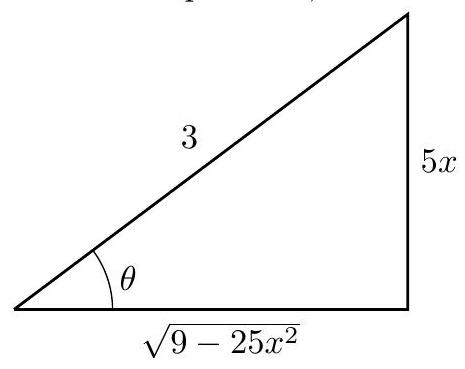
\includegraphics[max width=\textwidth, center]{2024_12_27_c5f2eac2dd536f5b8840g-14}

$$
\begin{aligned}
& \frac{3}{5} \sin \theta=x \\
& \frac{3}{5} \cos \theta \mathrm{~d} \theta=\mathrm{d} x \\
& 3 \cos \theta=\sqrt{9-25 x^{2}}
\end{aligned}
$$

We then compute

$$
\begin{aligned}
\int_{0}^{3 / 10} \frac{x^{2}}{\sqrt{9-25 x^{2}}} \mathrm{~d} x & =\int_{\arcsin (0)}^{\arcsin (1 / 2)} \frac{\left(\frac{3}{5} \sin \theta\right)^{2}}{3 \cos \theta} \frac{3}{5} \cos \theta \mathrm{~d} \theta \\
& =\frac{9}{125} \int_{0}^{\pi / 6} \sin ^{2} \theta \mathrm{~d} \theta \\
& =\frac{9}{250} \int_{0}^{\pi / 6}(1-\cos (2 \theta)) \mathrm{d} \theta \\
& =\frac{9}{250}\left[1-\frac{1}{2} \sin (2 \theta)\right]_{0}^{\pi / 6} \\
& =\frac{9}{250}\left(\frac{\pi}{6}-\frac{\sqrt{3}}{4}\right)=\frac{3}{1000}(2 \pi-3 \sqrt{3})
\end{aligned}
$$

(j) We consider the substitution $u=2 x^{2}-3$ so that $\mathrm{d} u=4 x \mathrm{~d} x$. Then

$$
\begin{aligned}
\int \frac{4 x^{5}}{\left(2 x^{2}-3\right)^{\frac{3}{2}}} \mathrm{~d} x & =\int \frac{x^{4}}{\left(2 x^{2}-3\right)^{\frac{3}{2}}} 4 x \mathrm{~d} x \\
& =\int \frac{\frac{1}{4}(u+3)^{2}}{(u)^{\frac{3}{2}}} \mathrm{~d} u \\
& =\frac{1}{4} \int \frac{u^{2}+6 u+9}{(u)^{\frac{3}{2}}} \mathrm{~d} u \\
& =\frac{1}{4} \int u^{1 / 2}+6 u^{-1 / 2}+9 u^{-3 / 2} \mathrm{~d} u \\
& =\frac{1}{4}\left(\frac{2}{3} u^{3 / 2}+12 u^{1 / 2}-18 u^{-1 / 2}\right)+C \\
& =\frac{1}{6}\left(\left(2 x^{2}-3\right)^{3 / 2}+18\left(2 x^{2}-3\right)^{1 / 2}-27\left(2 x^{2}-3\right)^{-1 / 2}\right)+C
\end{aligned}
$$

Multiplying and dividing by $\sqrt{2 x^{2}-3}$, we obtain a nicer expression:

$$
\begin{aligned}
\int \frac{4 x^{5}}{\left(2 x^{2}-3\right)^{\frac{3}{2}}} \mathrm{~d} x & =\frac{1}{6}\left(\frac{\left(2 x^{2}-3\right)^{2}+18\left(2 x^{2}-3\right)-27}{\sqrt{2 x^{2}-3}}\right)+C \\
& =\frac{1}{6}\left(\frac{4 x^{4}+24 x^{2}-72}{\sqrt{2 x^{2}-3}}\right)+C \\
& =\frac{2}{3}\left(\frac{x^{4}+6 x^{2}-18}{\sqrt{2 x^{2}-3}}\right)+C
\end{aligned}
$$

(k) We begin with the substitution $x=\cos (t)$ :

$$
\int_{0}^{\pi / 3} \frac{\sin (t) \cos (t)}{\sqrt{1+\cos ^{2}(t)}} \mathrm{d} t=-\int_{1}^{1 / 2} \frac{x}{\sqrt{1+x^{2}}} \mathrm{~d} x=\int_{1 / 2}^{1} \frac{x}{\sqrt{1+x^{2}}} \mathrm{~d} x
$$

We can then solve the integral with the substitution $u=1+x^{2}$. However, in order to provide another example with trigonometric substitution, we consider instead the substitution below.\\
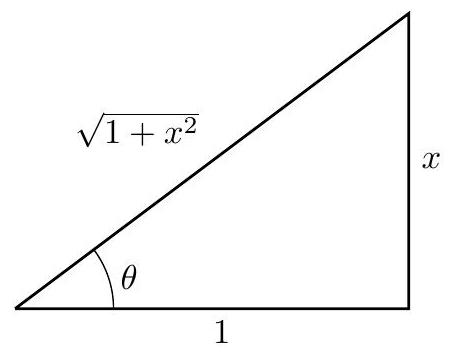
\includegraphics[max width=\textwidth, center]{2024_12_27_c5f2eac2dd536f5b8840g-16}

$$
\begin{aligned}
& \tan \theta=x \\
& \sec ^{2} \theta \mathrm{~d} \theta=\mathrm{d} x \\
& \sec \theta=\sqrt{1+x^{2}}
\end{aligned}
$$

We then have

$$
\begin{aligned}
\int_{0}^{\pi / 3} \frac{\sin (t) \cos (t)}{\sqrt{1+\cos ^{2}(t)}} \mathrm{d} t & =\int_{1 / 2}^{1} \frac{x}{\sqrt{1+x^{2}}} \mathrm{~d} x \\
& =\int_{\arctan (1 / 2)}^{\arctan (1)} \frac{\tan \theta}{\sec \theta} \sec ^{2} \theta \mathrm{~d} \theta \\
& =\int_{\arctan (/ 1 / 2)}^{\pi / 4} \sec \theta \tan \theta \mathrm{~d} \theta \\
& =\left.\sec \theta\right|_{\arctan (/ 1 / 2)} ^{\pi / 4} \\
& =\sqrt{2}-\sec (\arctan (1 / 2)) \\
& =\sqrt{2}-\frac{\sqrt{5}}{2}
\end{aligned}
$$

To find $\sec (\arctan (1 / 2))$, you can use trigonometric identities. For instance, noting that $\sec ^{2}(\arctan (1 / 2))=\tan ^{2}(\arctan (1 / 2))+1=\left(\frac{1}{2}\right)^{2}+1=\frac{5}{4}$ we can deduce $\sec (\arctan (1 / 2))=$ $\sqrt{5} / 2$.\\
(l) Recall that $\tan ^{2}(x)=\sec ^{2}(x)-1$ and

$$
\frac{\mathrm{d}}{\mathrm{~d} x} \tan (x)=\sec ^{2}(x)
$$

so that gives

$$
\int \tan ^{2}(x) d x=\int \sec ^{2}(x)-1 d x=\tan (x)-x+C
$$

(m) We proceed first by substitution, set $u:=x^{-1}$, then $\mathrm{d} u=-x^{-2}$, which gives us

$$
\int \frac{\sin ^{2}\left(\frac{1}{x}\right)}{x^{2}} d x=-\int \sin ^{2}(u) \mathrm{d} u
$$

We've already seen the integral of $\sin ^{2}(u)$ in class, so using that result we end with

$$
\int \frac{\sin ^{2}\left(\frac{1}{x}\right)}{x^{2}} d x=-\int \sin ^{2}(u) \mathrm{d} u=\frac{u}{2}-\frac{1}{4} \cos (2 u)+C=\frac{1}{2 x}-\frac{1}{4} \cos \left(\frac{2}{x}\right)+C
$$

(n) First we perform a substitution, then perform integration by parts twice. Start with setting $t:=\ln (x)$, then $x=e^{t}$ and $\mathrm{d} t=x^{-1} \mathrm{~d} x$, and

$$
\int\left(\frac{\ln (x)}{x}\right)^{2} d x=\int t^{2} e^{-t} d t
$$

Integration by parts once, with $u=t^{2}$ and $\mathrm{d} v=e^{-t} \mathrm{~d} t$ gives

$$
\int t^{2} e^{-t} d t=-t^{2} e^{-t}+2 \int t e^{-t} \mathrm{~d} t
$$

Finally, the second integration parts, this time with $u=t$ and $\mathrm{d} v=e^{-t} \mathrm{~d} t$ gives

$$
\int t e^{-t} \mathrm{~d} t=-t e^{-t}+\int e^{-t} \mathrm{~d} t=-t e^{-t}-e^{-t}
$$

Putting it all together, we end up with

$$
\int\left(\frac{\ln (x)}{x}\right)^{2} d x=-t^{2} e^{-t}+2\left(-t e^{-t}-e^{-t}\right)=-\frac{1}{x}\left((\ln (x))^{2}+2 \ln (x)+1\right) .
$$

\section*{Challenge Problems}
\begin{enumerate}
  \setcounter{enumi}{5}
  \item Prove that the following equation is correct for any continuously differentiable functions $f(x), g(x)$ and $h(x)$ :
\end{enumerate}

$$
\int_{a}^{b} f^{\prime}(x) g(x) h(x) d x=\left.f(x) g(x) h(x)\right|_{a} ^{b}-\int_{a}^{b} f(x) g^{\prime}(x) h(x) d x-\int_{a}^{b} f(x) g(x) h^{\prime}(x) d x
$$

\begin{enumerate}
  \setcounter{enumi}{6}
  \item Evaluate
\end{enumerate}

$$
\int_{-\pi}^{\pi} \arctan \left(\pi^{x}\right) \mathrm{d} x
$$

Hint: consider using the substitution $u:=-x$. You might need the identity

$$
\arctan (1 / s)=\operatorname{arccot}(s)=\frac{\pi}{2}-\arctan (s)
$$

where the first equality is valid for $s>0$.\\
8. Compute the following integral with the appropriate method(s)

$$
\int \frac{x \ln (x)}{\sqrt{x^{2}-1}} \mathrm{~d} x
$$

Hint: start with integration by parts.\\
9. (a) Using trigonometric substitution show that

$$
\int \frac{\mathrm{d} x}{\sqrt{x^{2}+a^{2}}}=\ln \left(x+\sqrt{x^{2}+a^{2}}\right)+C .
$$

(b) Use the hyperbolic substitution $x=a \cdot \sinh (t)$ to show that

$$
\int \frac{\mathrm{d} x}{\sqrt{x^{2}+a^{2}}}=\operatorname{arcsinh}\left(\frac{x}{a}\right)+C
$$

where $a>0$ is a constant.\\
(c) Using part (a), provide an expression for $\operatorname{arcsinh}\left(\frac{x}{a}\right)$ in terms of the logarithm function.

Recall: $\cosh ^{2}(\phi)=1+\sinh ^{2}(\phi)$ and $\cosh (x)>0$ for all $x \in \mathbb{R}$.


\end{document}